\documentclass[11pt,a4paper]{article}

% --- Packages ---
\usepackage[a4paper,margin=1in]{geometry}
\usepackage{microtype}
\usepackage{graphicx}
\usepackage{amsmath,amssymb}
\usepackage{booktabs}
\usepackage{tabularx}
\usepackage{array}
\usepackage{caption}
\usepackage{subcaption}
\usepackage{xcolor}
\usepackage{enumitem}
\usepackage{tikz}
\usepackage{pgfplots}
\usepackage{hyperref}
\usepackage{url}
\usepackage{cite}

% --- TikZ & PGFPlots Settings ---
\pgfplotsset{compat=1.18}
\usetikzlibrary{shapes.geometric, arrows.meta, positioning, calc, backgrounds, fit}

% --- Hyperlink Settings ---
\hypersetup{
  colorlinks=true,
  linkcolor=blue!70!black,
  citecolor=blue!70!black,
  urlcolor=blue!70!black
}

% --- Document Metadata ---
\title{\textbf{Comparative Performance Evaluation of Lexical, Semantic, and Hybrid Retrieval for Duplicate Question Retrieval}}

\author{
  \textbf{Student Name} \\
  Registration Number: \texttt{[REG-XXXXXX]} \\
  Department of Computer Science and Engineering \\
  \texttt{student@institution.edu}
}
\date{\today}

\begin{document}
\maketitle

\begin{abstract}
Duplicate question retrieval is a foundational challenge in large-scale Community Question Answering (CQA) platforms, where recurring queries fragment user attention and dilute repository knowledge. In this work, we design, implement, and empirically evaluate a complete Information Retrieval (IR) pipeline for duplicate question search using the Quora Question Pairs (QQP) dataset. We transform 404,268 pairwise annotations into an ad-hoc retrieval corpus of 537,905 unique questions and establish ground-truth relevance clusters using graph-theoretic transitive closure over connected components ($N=60,449$ components). This partitioning enforces strict component-level isolation between training, validation, and testing splits, eliminating evaluation data leakage. We implement and benchmark four distinct retrieval systems under an identical protocol: sublinear TF-IDF sparse cosine retrieval, Okapi BM25, dense semantic bi-encoder retrieval using Sentence-BERT (\texttt{all-MiniLM-L6-v2}), and a hybrid Reciprocal Rank Fusion (RRF, $k=60$) architecture. On 1,000 unseen test queries, SBERT achieves the strongest overall ranking quality with MAP@10 of 0.7036 and nDCG@10 of 0.7774 at 44.0\,ms median latency, substantially outperforming BM25 (MAP@10 0.5965) and TF-IDF (MAP@10 0.5955). Hybrid RRF successfully fuses ranking signals to yield a balanced Recall@10 of 0.7538 and nDCG@10 of 0.7469. We deploy the pipeline into an interactive search engine and open-source the complete reproducible benchmark and automated test suite.
\end{abstract}

\vspace{0.5em}
\noindent\textbf{Keywords:}
Information Retrieval; Duplicate Question Retrieval; Quora Question Pairs; TF-IDF; BM25; Sentence Transformers; Reciprocal Rank Fusion; Semantic Search; MAP; nDCG.

\newpage

% =========================================================================
% SECTION 1: INTRODUCTION
% =========================================================================
\section{Introduction}
\label{sec:introduction}

Community Question Answering (CQA) platforms such as Quora, Stack Overflow, and Reddit process millions of user queries daily. A persistent operational challenge in these platforms is the recurring generation of duplicate questions---newly submitted inquiries that address the exact semantic intent of existing questions already answered in the knowledge base. Failing to identify and consolidate duplicate questions fragments community discussion, degrades retrieval relevance for subsequent users, and increases human moderation overhead. An effective duplicate question retrieval engine must dynamically surface identical questions from an existing corpus when a user enters a query into the search interface.

The core difficulty in duplicate question retrieval lies in the tension between \textit{lexical} and \textit{semantic} representations. Natural language provides vast combinatorial freedom to express the same underlying intent:
\begin{itemize}[noitemsep,topsep=0pt]
    \item \textbf{Vocabulary Mismatch and Paraphrasing:} Two questions may share virtually no identical lexical tokens while remaining semantically synonymous (e.g., \textit{``How can I earn cash over the internet?''} versus \textit{``What are effective ways to make money online?''}).
    \item \textbf{Surface Keyword Overlap with Differing Intent:} Conversely, two questions may share multiple high-frequency domain keywords while expressing contradictory or orthogonal objectives (e.g., \textit{``How do I install Python on Windows?''} versus \textit{``How do I uninstall Python from Windows?''}).
\end{itemize}

Traditional Information Retrieval models such as Term Frequency--Inverse Document Frequency (TF-IDF)~\cite{salton1988term} and the Okapi BM25 probabilistic model~\cite{robertson2009probabilistic} rely on sparse inverted index representations. They excel at exact keyword matching, offer sub-millisecond querying, and provide transparent scoring mechanics. However, because they assume term independence and lack semantic awareness, they suffer heavily from the vocabulary mismatch problem when questions are paraphrased.

Recent advances in neural representation learning, particularly transformer-based bi-encoders such as Sentence-BERT (SBERT)~\cite{reimers2019sentence}, map sentences into continuous, dense embedding spaces where cosine similarity reflects semantic relatedness. Bi-encoders enable fast vector retrieval by decoupling offline document encoding from online query processing. Nevertheless, dense semantic retrieval can exhibit failure modes: it may conflate general topical overlap with exact duplicate intent, or fail to register subtle polarity shifts introduced by negation particles (\textit{not}, \textit{never}, \textit{without}).

To leverage the complementary strengths of lexical precision and dense semantic coverage, rank fusion methods combine multiple candidate lists. Reciprocal Rank Fusion (RRF)~\cite{cormack2009reciprocal} provides an attractive mechanism because it fuses ordinal rank positions rather than attempting to normalize and calibrate disparate, non-commensurate raw scores (e.g., unbounded BM25 scores versus bounded cosine similarities).

In this study, we develop a comprehensive, end-to-end duplicate question retrieval engine evaluated on the Quora Question Pairs (QQP) dataset~\cite{iyer2017quora}. Unlike binary classification pipelines that merely predict whether a pre-paired tuple is duplicate, our system operates as an authentic information retrieval engine over a deduplicated corpus of 537,905 unique questions.

\subsection{Research Objectives and Contributions}
This project delivers the following primary contributions:
\begin{enumerate}[noitemsep,topsep=2pt]
    \item \textbf{Leakage-Free Retrieval Corpus Construction:} We transform 404,268 labeled question pairs into a corpus of 537,905 unique documents. By constructing an undirected graph of duplicate pairs and computing connected components via transitive closure, we partition the dataset into train (70\%), validation (15\%), and test (15\%) splits with mathematical guarantee of zero evaluation leakage across duplicate clusters.
    \item \textbf{Independent Implementation of Four Retrieval Paradigms:} We construct and optimize sparse TF-IDF cosine retrieval, Okapi BM25 with custom token preprocessing, dense bi-encoder SBERT retrieval (\texttt{all-MiniLM-L6-v2}), and a 3-way Reciprocal Rank Fusion (RRF) engine.
    \item \textbf{Conservative Preprocessing Strategy:} We implement a dual-track preprocessing pipeline: a conservative lexical normalizer that preserves crucial question interrogatives (\textit{how}, \textit{why}) and negations (\textit{not}, \textit{no}), alongside raw contextual text preservation for dense transformer encoders.
    \item \textbf{Empirical Evaluation Under Standardized Protocol:} We benchmark all four systems on 1,000 unseen test queries using Mean Average Precision (MAP@5, MAP@10), Normalized Discounted Cumulative Gain (nDCG@5, nDCG@10), Precision@K, Recall@K, and percentile latencies.
    \item \textbf{Interactive Web Application and Automated Suite:} We deploy a real-time Streamlit search interface with candidate ranking breakdown and consensus badges, backed by a comprehensive unit and integration test suite (22/22 passing tests).
\end{enumerate}

\newpage

% =========================================================================
% SECTION 2: ABOUT DATASET
% =========================================================================
\section{About Dataset}
\label{sec:dataset}

\subsection{Dataset Description}
We employ the official Quora Question Pairs (QQP) benchmark dataset released by Quora~\cite{iyer2017quora} and popularized in natural language understanding benchmarks such as GLUE~\cite{wang2018glue}. The raw dataset comprises 404,290 tab-separated rows. Each entry represents a question pair labeled by human community annotators with a binary indicator ($\mathtt{is\_duplicate} \in \{0, 1\}$).

Prior to corpus construction, we execute rigorous data hygiene checks:
\begin{itemize}[noitemsep,topsep=0pt]
    \item Dropped 3 malformed rows containing null values in either question field.
    \item Removed 19 exact self-duplicates where $\mathtt{question1}$ and $\mathtt{question2}$ were character-by-character identical.
\end{itemize}
The resulting cleaned dataset contains exactly 404,268 high-quality question pairs. Table~\ref{tab:qqp_schema} summarizes the dataset schema, and Table~\ref{tab:dataset_summary} reports overall corpus statistics.

\begin{table}[h]
\centering
\small
\caption{Quora Question Pairs (QQP) Dataset Schema.}
\label{tab:qqp_schema}
\begin{tabularx}{\textwidth}{llX}
\toprule
\textbf{Field} & \textbf{Data Type} & \textbf{Description} \\
\midrule
\texttt{id} & Integer & Unique sequential identifier for each annotated pair row. \\
\texttt{qid1} & Integer & Identifier corresponding to the first question in the pair. \\
\texttt{qid2} & Integer & Identifier corresponding to the second question in the pair. \\
\texttt{question1} & String & Raw text of the first question. \\
\texttt{question2} & String & Raw text of the second question. \\
\texttt{is\_duplicate} & Binary $\{0, 1\}$ & Ground truth label: 1 if semantically duplicate, 0 otherwise. \\
\bottomrule
\end{tabularx}
\end{table}

\begin{table}[h]
\centering
\small
\caption{Corpus and Graph Partitioning Summary Statistics.}
\label{tab:dataset_summary}
\begin{tabular}{llr}
\toprule
\textbf{Metric} & \textbf{Scope} & \textbf{Measured Count / Value} \\
\midrule
Raw Rows Downloaded & Original TSV & 404,290 \\
Cleaned Pair Rows & Null/Duplicate Filtered & 404,268 \\
Non-Duplicate Pairs ($\mathtt{is\_duplicate}=0$) & Cleaned Pairs & 255,019 (63.08\%) \\
Duplicate Pairs ($\mathtt{is\_duplicate}=1$) & Cleaned Pairs & 149,249 (36.92\%) \\
\midrule
Total Unique Questions ($N$) & Searchable Corpus & 537,905 \\
Duplicate Connected Components & Graph $G=(V, E)$ & 60,449 \\
Nodes in Duplicate Clusters & Transitive Closure Map & 149,628 \\
\midrule
Training Split Questions & 70\% Component Partition & 376,533 \\
Validation Split Questions & 15\% Component Partition & 80,686 \\
Test Split Questions & 15\% Component Partition & 80,686 \\
Evaluation Benchmark Queries & Unseen Test Queries & 1,000 \\
\bottomrule
\end{tabular}
\end{table}

\subsection{Pair Dataset versus Ad-Hoc Retrieval Corpus}
A standard misconception in literature is treating QQP purely as a pairwise binary classification task. In an operational search engine, the system does not receive pairs to classify; it receives a single natural-language query $q$ and must scan a massive collection $\mathcal{C}$ to retrieve the most relevant candidates.

To construct the searchable collection, we extract every unique question appearing in either $\mathtt{question1}$ or $\mathtt{question2}$. This yields an authoritative corpus of $N = 537,905$ unique documents. Each question is assigned a stable internal identifier ($\mathtt{qid}$).

\subsubsection{Transitive Closure and Duplicate Mapping}
Ground truth duplicate labels are inherently transitive: if question $A$ is duplicate to question $B$, and question $B$ is duplicate to question $C$, then $A$ and $C$ represent identical informational intent. We formalize this by defining an undirected graph $G = (V, E)$, where vertices $V$ represent question IDs and an edge $(u, v) \in E$ exists if $(u, v)$ was annotated with $\mathtt{is\_duplicate} = 1$.

We compute the connected components of $G$ using Breadth-First Search (BFS). This reveals 60,449 distinct connected components containing 149,628 unique questions. For each question $u$ belonging to component $\mathcal{K}$, its complete set of relevant ground-truth duplicates is:
\begin{equation}
\label{eq:duplicate_closure}
\mathcal{R}(u) = \mathcal{K} \setminus \{u\}
\end{equation}
Table~\ref{tab:illustrative_pairs} illustrates this transformation.

\begin{table}[h]
\centering
\small
\caption{Illustrative Transformation: Pair Rows to Transitive Duplicate Graph.}
\label{tab:illustrative_pairs}
\begin{tabularx}{\textwidth}{cccXcc}
\toprule
\textbf{Pair ID} & \textbf{qid1} & \textbf{qid2} & \textbf{Question Text (qid1 / qid2)} & \textbf{Label} & \textbf{Transitive Cluster} \\
\midrule
101 & 1 & 2 & \textit{How to learn Python?} / \textit{Best way to learn Python?} & 1 & $\{1, 2, 3\}$ \\
102 & 2 & 3 & \textit{Best way to learn Python?} / \textit{How do I start Python?} & 1 & $\{1, 2, 3\}$ \\
103 & 1 & 4 & \textit{How to learn Python?} / \textit{How to learn Java?} & 0 & Distinct ($\{4\}$) \\
\bottomrule
\end{tabularx}
\end{table}

\subsubsection{Caveat: Incomplete Relevance Judgments}
A critical reality of web-scale IR is that the absence of a labeled pair does \textbf{not} imply a confirmed negative. In QQP, annotators reviewed only a curated subset of pair candidates generated by Quora's internal retrieval heuristics. Consequently, if a model retrieves a relevant question that was never paired in the dataset, that candidate will be scored as non-relevant under binary evaluation. Thus, all empirical metrics reported in this study represent performance against \textit{known annotated positives}, representing a conservative lower bound on true retrieval utility.

\subsection{Dataset Visualizations}
Figure~\ref{fig:label_distribution} displays the class balance in the cleaned pair dataset, demonstrating that negative pairs constitute roughly 63\% of annotations. Figure~\ref{fig:question_lengths} plots the token length distribution across all 537,905 corpus questions. The distribution is right-skewed with a median length of 10 tokens and a 95th percentile of 22 tokens, highlighting that duplicate question retrieval is fundamentally a short-text retrieval challenge where document-length normalization requires delicate tuning.

\begin{figure}[t]
\centering
\begin{subfigure}[b]{0.48\textwidth}
    \centering
    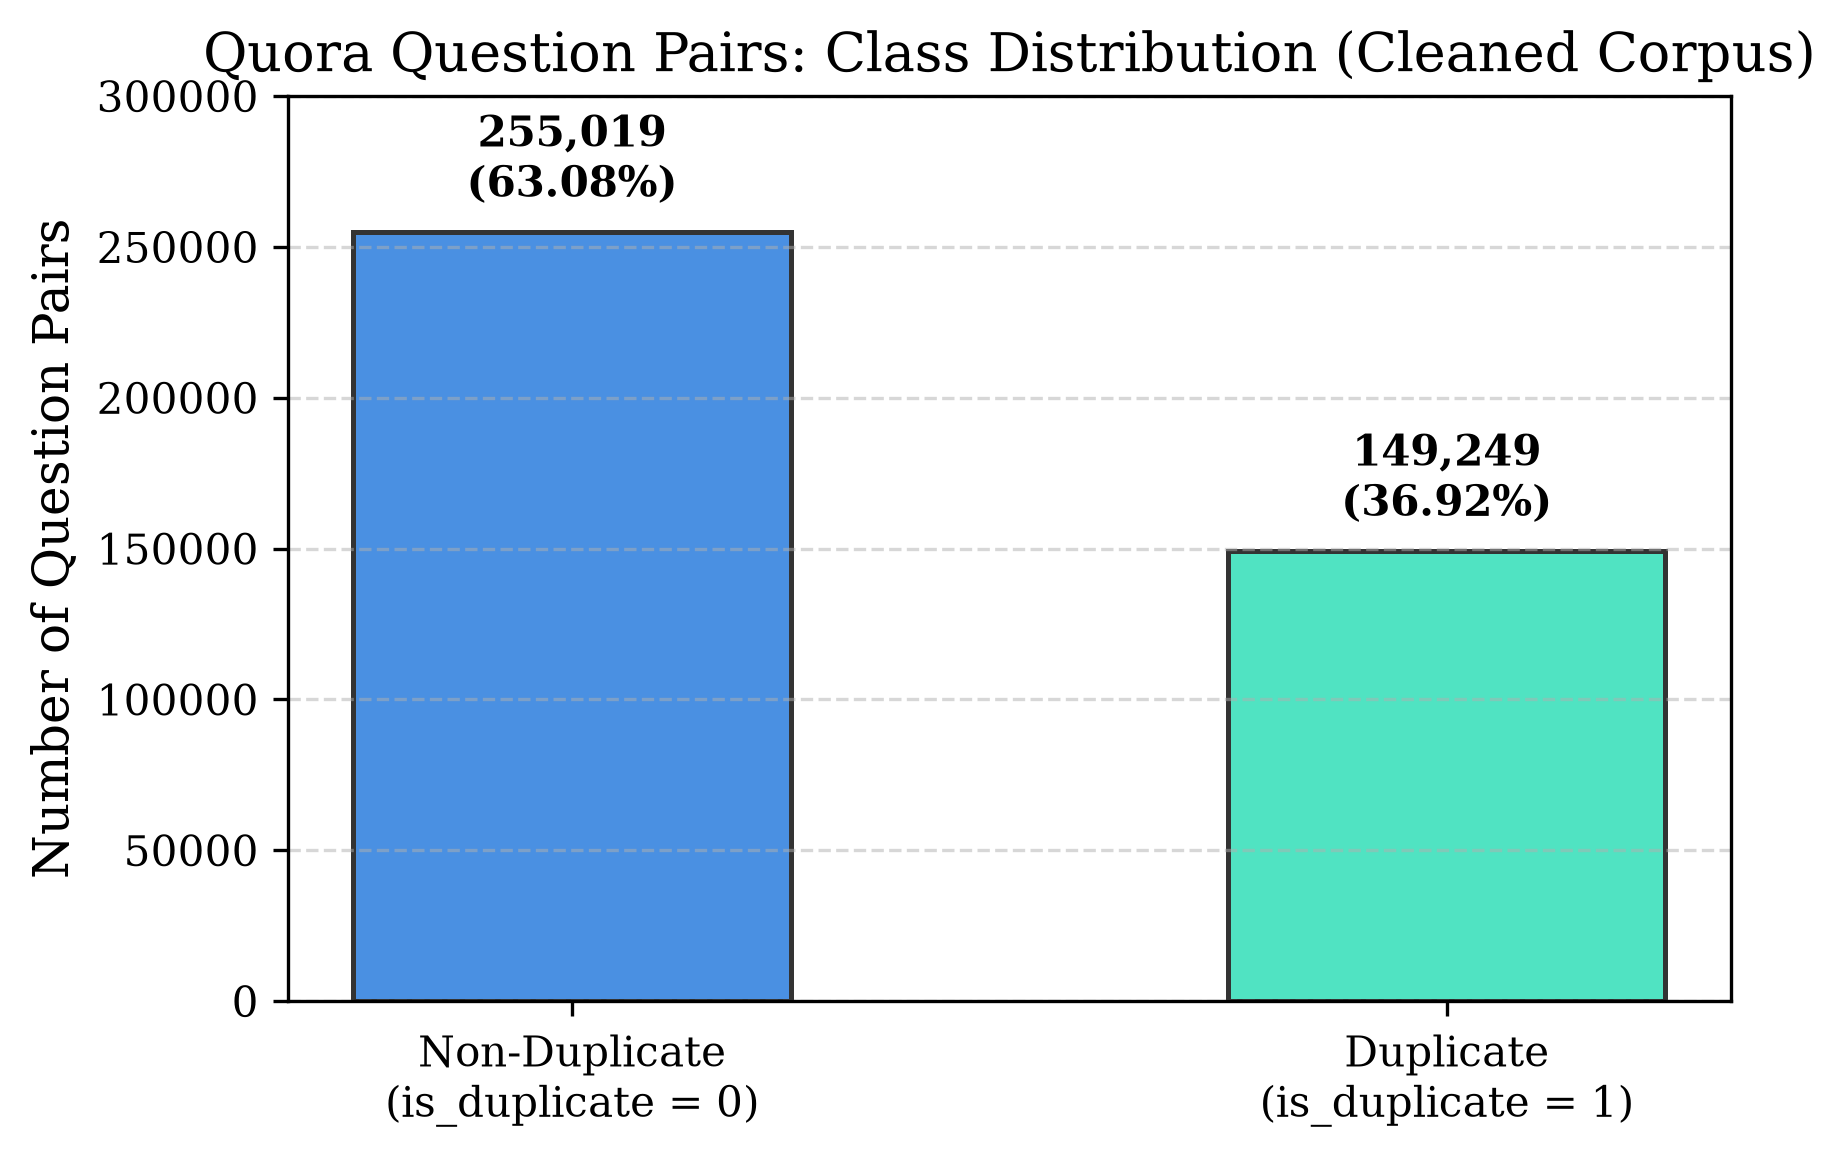
\includegraphics[width=\textwidth]{figures/label_distribution.png}
    \caption{Class distribution of cleaned QQP pairs.}
    \label{fig:label_distribution}
\end{subfigure}
\hfill
\begin{subfigure}[b]{0.48\textwidth}
    \centering
    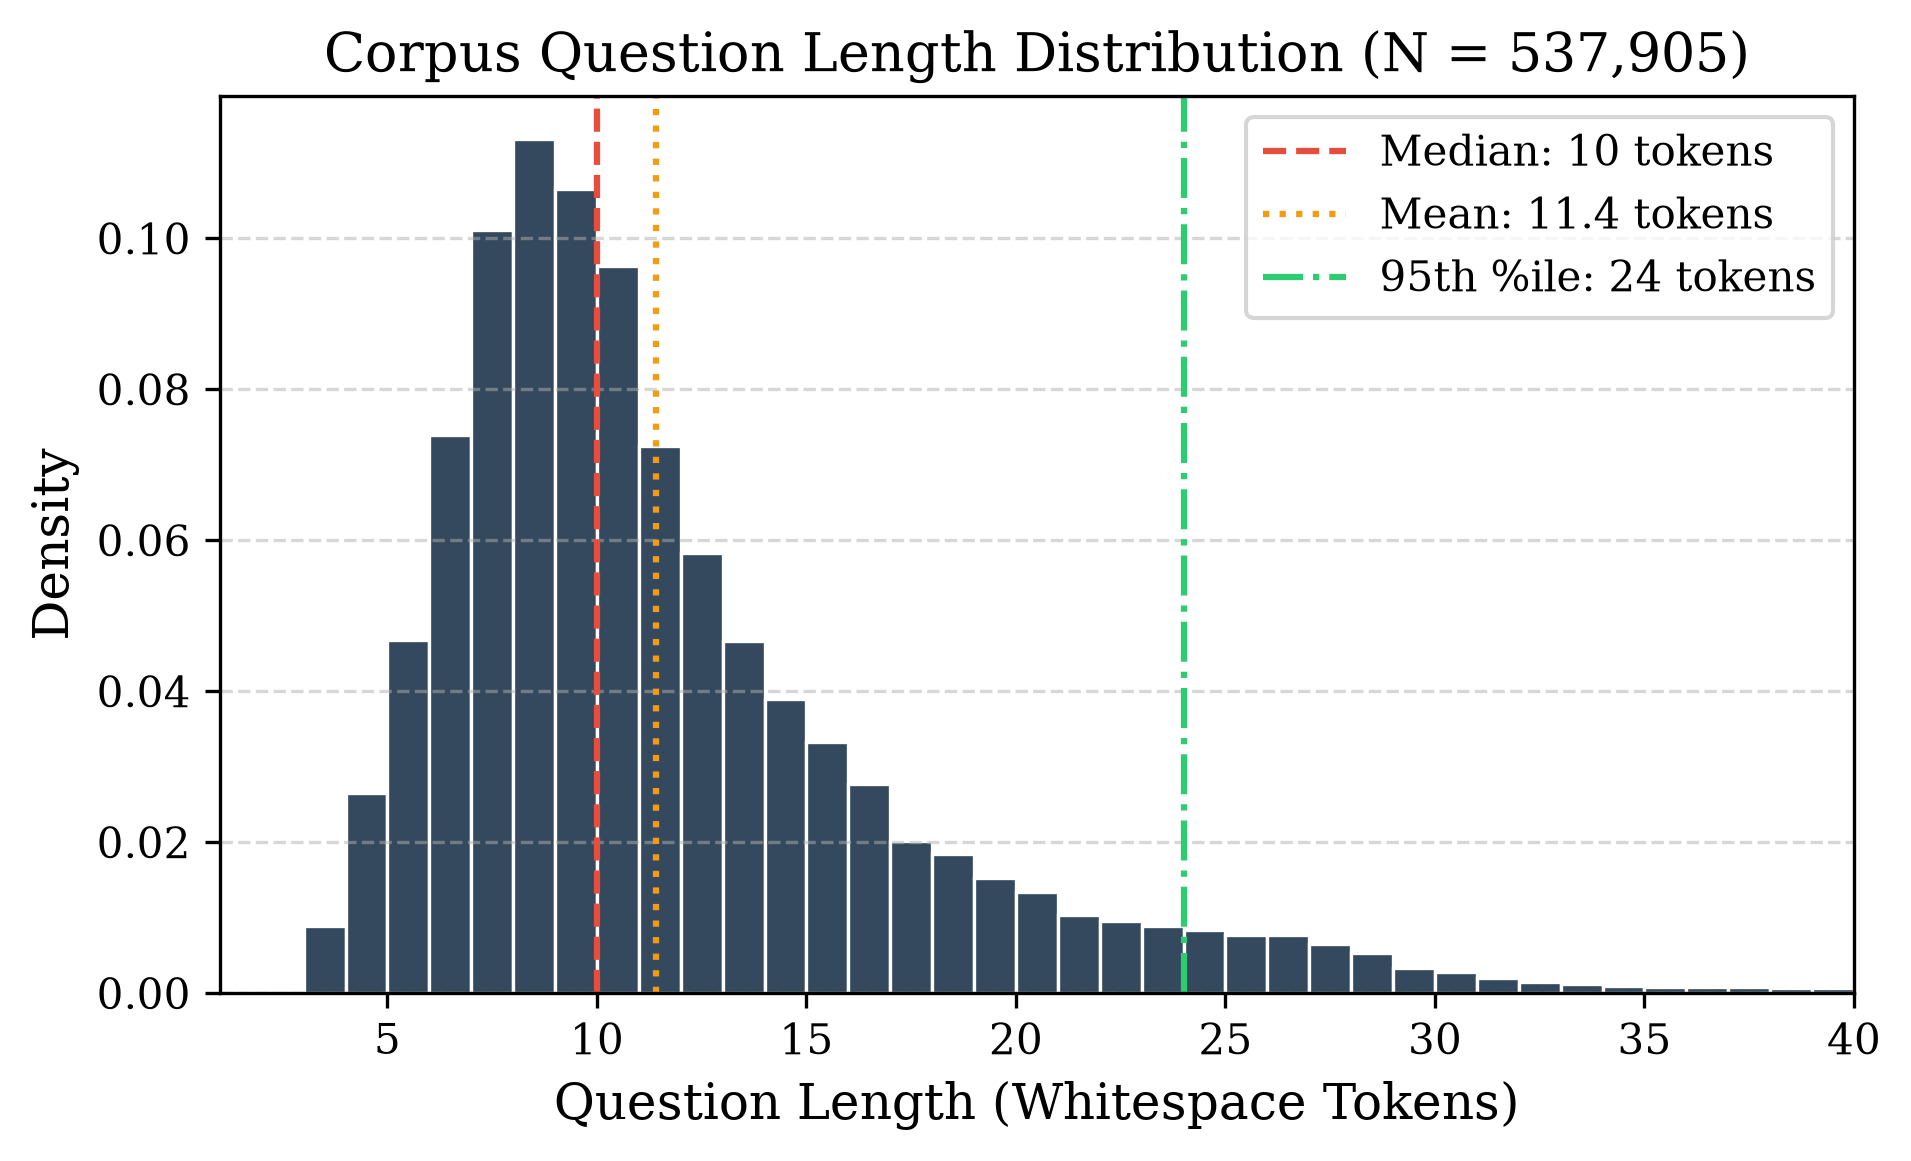
\includegraphics[width=\textwidth]{figures/question_lengths.png}
    \caption{Question token length distribution ($N=537,905$).}
    \label{fig:question_lengths}
\end{subfigure}
\caption{Exploratory data analysis of the Quora Question Pairs corpus.}
\label{fig:dataset_eda}
\end{figure}

\newpage

% =========================================================================
% SECTION 3: METHODOLOGY
% =========================================================================
\section{Methodology}
\label{sec:methodology}

\subsection{System Architecture}
The system separates heavy offline index construction from low-latency online query processing. Figure~\ref{fig:architecture} illustrates the end-to-end architecture.

\begin{figure}[h]
\centering
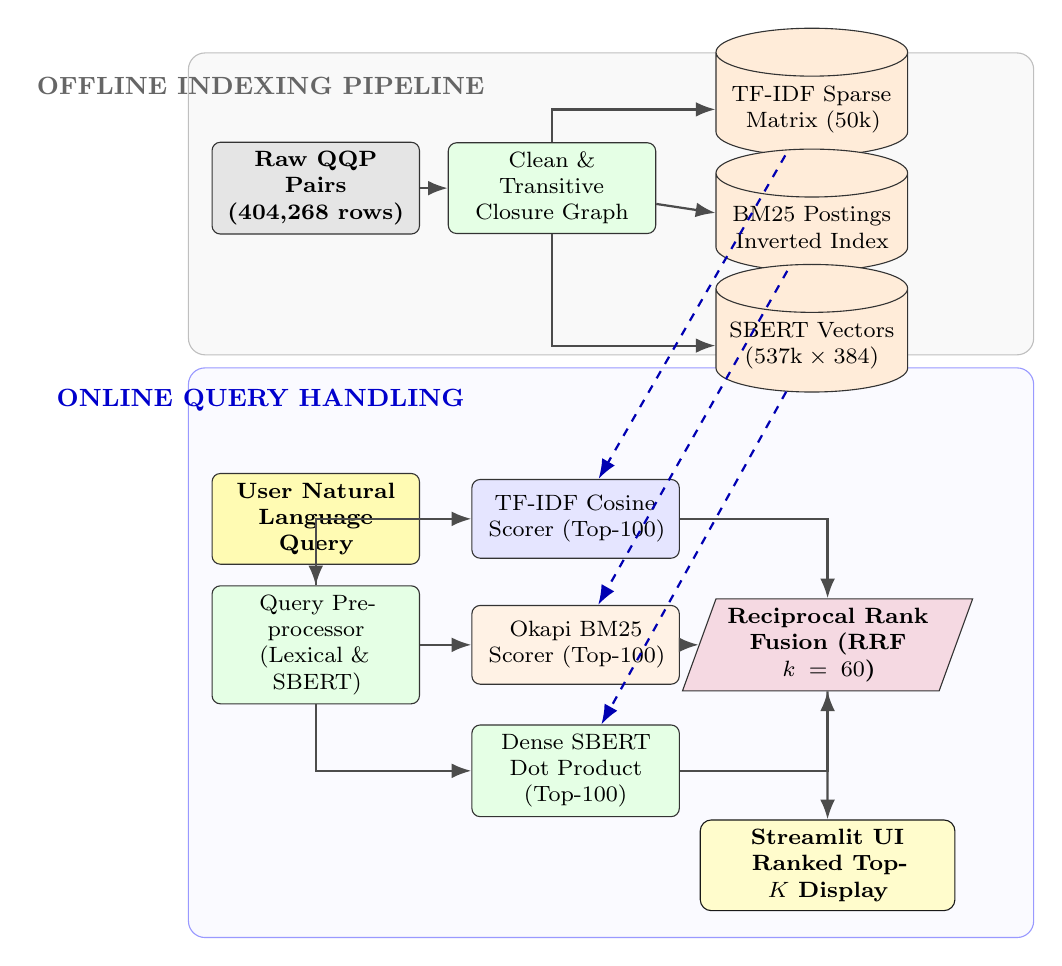
\begin{tikzpicture}[
    node distance=1.3cm and 1.0cm,
    box/.style={rectangle, draw=black!80, fill=blue!8, rounded corners=3pt, text width=2.4cm, minimum height=1.0cm, align=center, font=\footnotesize\bfseries},
    proc/.style={rectangle, draw=black!80, fill=green!10, rounded corners=3pt, text width=2.4cm, minimum height=1.0cm, align=center, font=\footnotesize},
    idx/.style={cylinder, draw=black!80, shape border rotate=90, aspect=0.25, fill=orange!15, text width=2.2cm, minimum height=1.2cm, align=center, font=\footnotesize},
    fuse/.style={trapezium, trapezium left angle=70, trapezium right angle=110, draw=black!80, fill=purple!15, text width=2.6cm, minimum height=1.0cm, align=center, font=\footnotesize\bfseries},
    ui/.style={rectangle, draw=black!90, fill=yellow!20, rounded corners=4pt, text width=3.0cm, minimum height=1.0cm, align=center, font=\footnotesize\bfseries},
    arrow/.style={-{Latex[length=2.5mm]}, thick, draw=black!70},
    dasharrow/.style={-{Latex[length=2.5mm]}, thick, dashed, draw=blue!70!black}
]

% Background panels
\begin{scope}[on background layer]
    \node (offbox) [draw=gray!50, fill=gray!5, rounded corners=6pt, fit={(0,4.8) (10.5,1.2)}] {};
    \node at (0.8,4.5) [font=\small\bfseries\color{gray!80!black}] {OFFLINE INDEXING PIPELINE};

    \node (onbox) [draw=blue!40, fill=blue!2, rounded corners=6pt, fit={(0,0.8) (10.5,-6.2)}] {};
    \node at (0.8,0.5) [font=\small\bfseries\color{blue!80!black}] {ONLINE QUERY HANDLING};
\end{scope}

% Offline Nodes
\node (raw) at (1.5, 3.2) [box, fill=gray!20] {Raw QQP Pairs\\(404,268 rows)};
\node (corpus) at (4.5, 3.2) [proc] {Clean \& Transitive\\Closure Graph};
\node (tfidf_idx) at (7.8, 4.2) [idx] {TF-IDF Sparse\\Matrix ($50\text{k}$)};
\node (bm25_idx) at (7.8, 2.7) [idx] {BM25 Postings\\Inverted Index};
\node (sbert_idx) at (7.8, 1.2) [idx] {SBERT Vectors\\($537\text{k}\times 384$)};

% Online Nodes
\node (query) at (1.5, -1.0) [box, fill=yellow!30] {User Natural\\Language Query};
\node (preproc) at (1.5, -2.6) [proc] {Query Preprocessor\\(Lexical \& SBERT)};

\node (tfidf_ret) at (4.8, -1.0) [proc, fill=blue!10] {TF-IDF Cosine\\Scorer (Top-100)};
\node (bm25_ret) at (4.8, -2.6) [proc, fill=orange!10] {Okapi BM25\\Scorer (Top-100)};
\node (sbert_ret) at (4.8, -4.2) [proc, fill=green!10] {Dense SBERT\\Dot Product (Top-100)};

\node (rrf) at (8.0, -2.6) [fuse] {Reciprocal Rank\\Fusion (RRF $k=60$)};
\node (ui_node) at (8.0, -5.4) [ui] {Streamlit UI\\Ranked Top-$K$ Display};

% Arrows Offline
\draw [arrow] (raw) -- (corpus);
\draw [arrow] (corpus) |- (tfidf_idx);
\draw [arrow] (corpus) -- (bm25_idx);
\draw [arrow] (corpus) |- (sbert_idx);

% Arrows Online
\draw [arrow] (query) -- (preproc);
\draw [arrow] (preproc) |- (tfidf_ret);
\draw [arrow] (preproc) -- (bm25_ret);
\draw [arrow] (preproc) |- (sbert_ret);

% Index connections
\draw [dasharrow] (tfidf_idx) -- (tfidf_ret);
\draw [dasharrow] (bm25_idx) -- (bm25_ret);
\draw [dasharrow] (sbert_idx) -- (sbert_ret);

% Fusion and Output
\draw [arrow] (tfidf_ret) -| (rrf);
\draw [arrow] (bm25_ret) -- (rrf);
\draw [arrow] (sbert_ret) -| (rrf);
\draw [arrow] (rrf) -- (ui_node);

\end{tikzpicture}
\caption{System architecture separating offline corpus indexing from online multi-retriever query processing and Reciprocal Rank Fusion.}
\label{fig:architecture}
\end{figure}

\subsection{Preprocessing and Corpus Construction}
Standard aggressive text normalization pipelines strip punctuation, numbers, and stopwords indiscriminately. For duplicate question retrieval, such aggressive pruning is catastrophic:
\begin{itemize}[noitemsep,topsep=0pt]
    \item \textbf{Negation Inversion:} Removing words like \textit{not}, \textit{no}, or \textit{never} flips query polarity, causing non-duplicates to appear identical (e.g., \textit{``Why should I not buy an iPhone?''} vs. \textit{``Why should I buy an iPhone?''}).
    \item \textbf{Interrogative Intent:} Stripping question interrogatives (\textit{how}, \textit{why}, \textit{what}, \textit{where}) destroys intent differentiation (e.g., \textit{``How to make pizza?''} vs. \textit{``Where to buy pizza?''}).
\end{itemize}

To prevent these pitfalls, we designed a \textbf{conservative lexical preprocessor}:
\begin{enumerate}[noitemsep,topsep=1pt]
    \item Lowercase ASCII normalization and whitespace trimming.
    \item Contraction expansion mapping 28 common English contractions (e.g., \textit{can't $\to$ cannot}, \textit{won't $\to$ will not}, \textit{how's $\to$ how is}).
    \item Punctuation stripping with special handling to retain negation morphemes.
    \item Stopword filtering based on standard NLTK English stopwords, but with a strict preservation whitelist containing all negation words (\textit{not}, \textit{no}, \textit{nor}, \textit{never}, \textit{neither}, \textit{cannot}, \textit{without}) and interrogative markers (\textit{how}, \textit{why}, \textit{what}, \textit{which}, \textit{who}, \textit{whom}, \textit{where}, \textit{when}).
    \item Porter stemming~\cite{manning2008introduction} for lexical term conflation.
\end{enumerate}

For the dense transformer model, we deploy a separate preprocessor that preserves raw case, punctuation, and word order, as pretrained transformer tokenizers rely on subword positional context.

\subsubsection{Leakage-Free Component Splitting}
A pervasive error in CQA benchmarks is random pair-level splitting. If question $A$ and $B$ are in the training set, but question $B$ and $C$ appear in the test set, the model effectively memorizes the semantic cluster during training, falsely inflating evaluation scores.

To achieve strict evaluation hygiene, we partition the dataset at the \textbf{connected-component level}. We assign 70\% of connected components to training (376,533 questions), 15\% to validation (80,686 questions), and 15\% to testing (80,686 questions). This guarantees that no question in the test set shares an edge or transitive connection with any question in the training set.

\subsection{TF-IDF Retrieval}
We map each question into a high-dimensional vector space $\mathbb{R}^{|V|}$ where $|V| = 50,000$. To reduce the distortion caused by highly frequent terms, we employ sublinear term frequency scaling:
\begin{equation}
\operatorname{tf}(t, d) = \begin{cases} 
1 + \log(f_{t, d}), & \text{if } f_{t, d} > 0 \\ 
0, & \text{otherwise} 
\end{cases}
\end{equation}
We apply scikit-learn's smoothed inverse document frequency~\cite{pedregosa2011scikit}:
\begin{equation}
\operatorname{idf}(t) = \log\left(\frac{1 + N}{1 + \operatorname{df}(t)}\right) + 1
\end{equation}
Each document vector is $L_2$-normalized:
\begin{equation}
\mathbf{v}_d = \frac{\mathbf{w}_d}{\|\mathbf{w}_d\|_2}, \quad \text{where } w_{t, d} = \operatorname{tf}(t, d) \cdot \operatorname{idf}(t)
\end{equation}
Online ranking computes the cosine similarity against the normalized query vector $\mathbf{v}_q$ via sparse matrix-vector multiplication:
\begin{equation}
\operatorname{score}_{\text{TF-IDF}}(q, d) = \mathbf{v}_q^\top \mathbf{v}_d = \sum_{t \in q \cap d} v_{t, q} \cdot v_{t, d}
\end{equation}

\subsection{BM25 Retrieval}
Okapi BM25~\cite{robertson2009probabilistic} refines term weighting by introducing non-linear term frequency saturation and document length normalization. Given query $Q = (q_1, q_2, \dots, q_m)$ and document $D$:
\begin{equation}
\operatorname{score}_{\text{BM25}}(Q, D) = \sum_{i=1}^{m} \operatorname{IDF}(q_i) \cdot \frac{f(q_i, D) \cdot (k_1 + 1)}{f(q_i, D) + k_1 \cdot \left(1 - b + b \cdot \frac{|D|}{\operatorname{avgdl}}\right)}
\end{equation}
where $f(q_i, D)$ is the raw term frequency, $|D|$ is the token length of document $D$, and $\operatorname{avgdl}$ is the average document length across the corpus ($\operatorname{avgdl} \approx 10.95$ tokens). The inverse document frequency is defined as:
\begin{equation}
\operatorname{IDF}(q_i) = \log\left(\frac{N - n(q_i) + 0.5}{n(q_i) + 0.5} + 1\right)
\end{equation}
We configure standard parameters $k_1 = 1.5$ (term frequency saturation limit) and $b = 0.75$ (length penalty). We maintain an in-memory inverted index mapping stemmed tokens to postings lists.

\subsection{Sentence Transformer Dense Semantic Retrieval}
For semantic retrieval, we utilize \texttt{sentence-transformers/all-MiniLM-L6-v2}~\cite{reimers2019sentence}, a 6-layer MiniLM bi-encoder with hidden dimension $d = 384$. The model maps input text into a contextual sequence of hidden states $\mathbf{h}_1, \dots, \mathbf{h}_T$ and computes the sentence representation via mean pooling over attention-masked token states:
\begin{equation}
\mathbf{u} = \frac{\sum_{i=1}^T m_i \mathbf{h}_i}{\sum_{i=1}^T m_i}, \quad \mathbf{e} = \frac{\mathbf{u}}{\|\mathbf{u}\|_2}
\end{equation}
Offline, we encode all 537,905 questions using PyTorch with CUDA acceleration on an NVIDIA GeForce RTX 4060 GPU (batch size 512). The resulting $537,905 \times 384$ single-precision float32 matrix occupies 826.2\,MB on disk.

Because all corpus vectors are pre-normalized ($\|\mathbf{e}_d\|_2 = 1$), online retrieval for a normalized query vector $\mathbf{e}_q$ reduces to a matrix-vector dot product:
\begin{equation}
\operatorname{score}_{\text{SBERT}}(q, d) = \mathbf{e}_q^\top \mathbf{e}_d = \sum_{j=1}^{384} e_{q, j} \cdot e_{d, j}
\end{equation}
Top candidates are extracted using partial top-$K$ selection via \texttt{numpy.argpartition}. For deployment resilience, the retriever includes automatic fallback to CPU inference if CUDA memory allocation encounters contention.

\subsection{Reciprocal Rank Fusion (RRF)}
When combining disparate retrieval engines, linear score combination is problematic because lexical scores (BM25 $\in [0, \infty)$) and dense similarity scores (cosine $\in [-1, 1]$) follow completely different distributions and cannot be normalized reliably across diverse query types.

Reciprocal Rank Fusion (RRF)~\cite{cormack2009reciprocal} solves this by fusing the ordinal rankings produced by individual retrievers. For a set of retrieval models $\mathcal{M} = \{\text{TF-IDF}, \text{BM25}, \text{SBERT}\}$ and a candidate document $d$:
\begin{equation}
\label{eq:rrf_formula}
\operatorname{RRF}(d) = \sum_{m \in \mathcal{M}} \frac{1}{k + r_m(d)}
\end{equation}
where $r_m(d) \in \{1, 2, \dots, K_{\text{pool}}\}$ represents the 1-based rank position of candidate $d$ in system $m$. We configure the smoothing constant $k = 60$ as empirically recommended in IR literature~\cite{cormack2009reciprocal}. If candidate $d$ is absent from the top-$K_{\text{pool}}$ ($K_{\text{pool}} = 100$) retrieved candidates of model $m$, its contribution from that model is 0. Candidates are sorted descending by $\operatorname{RRF}(d)$, with deterministic tie-breaking based on minimum rank.

\subsection{Implementation Stack}
Table~\ref{tab:tech_stack} details the software libraries and architectural roles supporting the pipeline.

\begin{table}[h]
\centering
\small
\caption{Technology Stack and Architectural Component Roles.}
\label{tab:tech_stack}
\begin{tabularx}{\textwidth}{llX}
\toprule
\textbf{Component / Library} & \textbf{Version} & \textbf{System Role and Responsibility} \\
\midrule
Python & 3.13.5 & Core runtime environment. \\
PyTorch & 2.14.1+cu126 & Tensor computation with CUDA 12.6 acceleration. \\
Sentence-Transformers & 3.4.1 & Bi-encoder model architecture (\texttt{all-MiniLM-L6-v2}). \\
Scikit-learn & 1.6.1 & Sparse TF-IDF vectorization and cosine dot products. \\
rank\_bm25 & 0.2.2 & Inverted index Okapi BM25 implementation. \\
NumPy \& Pandas & 2.2.3 / 2.2.3 & Matrix algebra, tabular serialization, and data hygiene. \\
Matplotlib & 3.10.1 & Publication plotting (PR curves, latency trade-offs). \\
Streamlit & 1.42.0 & Interactive real-time search interface and analytics UI. \\
Pytest & 9.1.1 & Automated unit and integration test framework. \\
\bottomrule
\end{tabularx}
\end{table}

\newpage

% =========================================================================
% SECTION 4: EXPERIMENTAL SETUP AND PERFORMANCE ANALYSIS
% =========================================================================
\section{Experimental Setup and Performance Analysis}
\label{sec:experiments}

\subsection{Experimental Setup}
Evaluation is conducted on $N_{\text{eval}} = 1,000$ unseen query questions randomly sampled from the held-out test split. To ensure rigorous evaluation:
\begin{enumerate}[noitemsep,topsep=1pt]
    \item Every test query is guaranteed to possess at least one confirmed duplicate in the corpus ($\mathcal{R}(q) \ge 1$).
    \item \textbf{Self-Exclusion Policy:} A query question is strictly prohibited from retrieving itself ($\operatorname{qid}_d \ne \operatorname{qid}_q$).
    \item Evaluation is executed over the full $N = 537,905$ question corpus.
    \item Queries are processed individually to measure realistic single-user latency.
\end{enumerate}
All experiments were conducted on an Intel Core i7 system equipped with 16\,GB RAM and an NVIDIA GeForce RTX 4060 Laptop GPU (8\,GB VRAM) under Windows 11.

\subsection{Evaluation Metrics}
We report standard Information Retrieval metrics matching our exact mathematical implementation:

\subsubsection{Precision@K and Recall@K}
For a cutoff $K$, let $\mathcal{S}_K(q)$ denote the set of top-$K$ retrieved candidate question IDs, and $\mathcal{R}(q)$ denote the ground-truth duplicate set:
\begin{equation}
P@K(q) = \frac{|\mathcal{S}_K(q) \cap \mathcal{R}(q)|}{K}
\end{equation}
\begin{equation}
R@K(q) = \frac{|\mathcal{S}_K(q) \cap \mathcal{R}(q)|}{|\mathcal{R}(q)|}
\end{equation}

\subsubsection{Average Precision and Mean Average Precision (MAP@K)}
Average Precision at cutoff $K$ rewards systems that place relevant items at higher rank positions:
\begin{equation}
\operatorname{AP}@K(q) = \frac{1}{\min(|\mathcal{R}(q)|, K)} \sum_{i=1}^{K} P@i(q) \cdot \operatorname{rel}_i
\end{equation}
where $\operatorname{rel}_i \in \{0, 1\}$ is the binary relevance indicator of the document at rank $i$. Mean Average Precision is the macro-average across all evaluation queries $Q_{\text{eval}}$:
\begin{equation}
\operatorname{MAP}@K = \frac{1}{|Q_{\text{eval}}|} \sum_{q \in Q_{\text{eval}}} \operatorname{AP}@K(q)
\end{equation}

\subsubsection{Discounted Cumulative Gain (nDCG@K)}
Discounted Cumulative Gain introduces a logarithmic penalty for relevant documents retrieved at deeper ranks:
\begin{equation}
\operatorname{DCG}@K(q) = \sum_{i=1}^{K} \frac{2^{\operatorname{rel}_i} - 1}{\log_2(i + 1)}
\end{equation}
The Normalized Discounted Cumulative Gain normalizes by the Ideal DCG ($\operatorname{IDCG}@K$), representing the score achieved under perfect ranking:
\begin{equation}
\operatorname{nDCG}@K(q) = \frac{\operatorname{DCG}@K(q)}{\operatorname{IDCG}@K(q)}, \quad \operatorname{nDCG}@K = \frac{1}{|Q_{\text{eval}}|} \sum_{q \in Q_{\text{eval}}} \operatorname{nDCG}@K(q)
\end{equation}

\subsection{Quantitative Comparison}
Table~\ref{tab:model_comparison} reports the comprehensive benchmark results across all four retrieval engines on the 1,000 unseen test queries.

\begin{table}[h]
\centering
\small
\caption{Empirical Performance Comparison Across Retrieval Paradigms on 1,000 Unseen Test Queries ($N_{\text{corpus}} = 537,905$). Best results in \textbf{bold}; second-best \underline{underlined}.}
\label{tab:model_comparison}
\begin{tabularx}{\textwidth}{lcccccccc}
\toprule
\textbf{Retriever} & \textbf{MAP@5} & \textbf{MAP@10} & \textbf{nDCG@5} & \textbf{nDCG@10} & \textbf{P@10} & \textbf{R@10} & \textbf{p50 Lat.} & \textbf{Mean Lat.} \\
\midrule
TF-IDF & 0.6047 & 0.5955 & 0.6699 & 0.6800 & 0.2231 & 0.6977 & 100.0\,ms & 108.7\,ms \\
BM25 & 0.6039 & 0.5965 & 0.6688 & 0.6811 & 0.2247 & 0.7051 & 795.0\,ms & 870.4\,ms \\
SBERT & \textbf{0.7078} & \textbf{0.7036} & \textbf{0.7653} & \textbf{0.7774} & \textbf{0.2716} & \textbf{0.7786} & \textbf{44.0\,ms} & \underline{118.6\,ms} \\
Hybrid RRF & \underline{0.6765} & \underline{0.6657} & \underline{0.7386} & \underline{0.7469} & \underline{0.2538} & \underline{0.7538} & 981.5\,ms & 1,048.5\,ms \\
\bottomrule
\end{tabularx}
\end{table}

\subsection{Precision--Recall Analysis}
Figure~\ref{fig:pr_curve} displays the cutoff-based retrieval Precision--Recall curves across cutoffs $K \in [1, 30]$. 

\begin{figure}[t]
\centering
\begin{subfigure}[b]{0.48\textwidth}
    \centering
    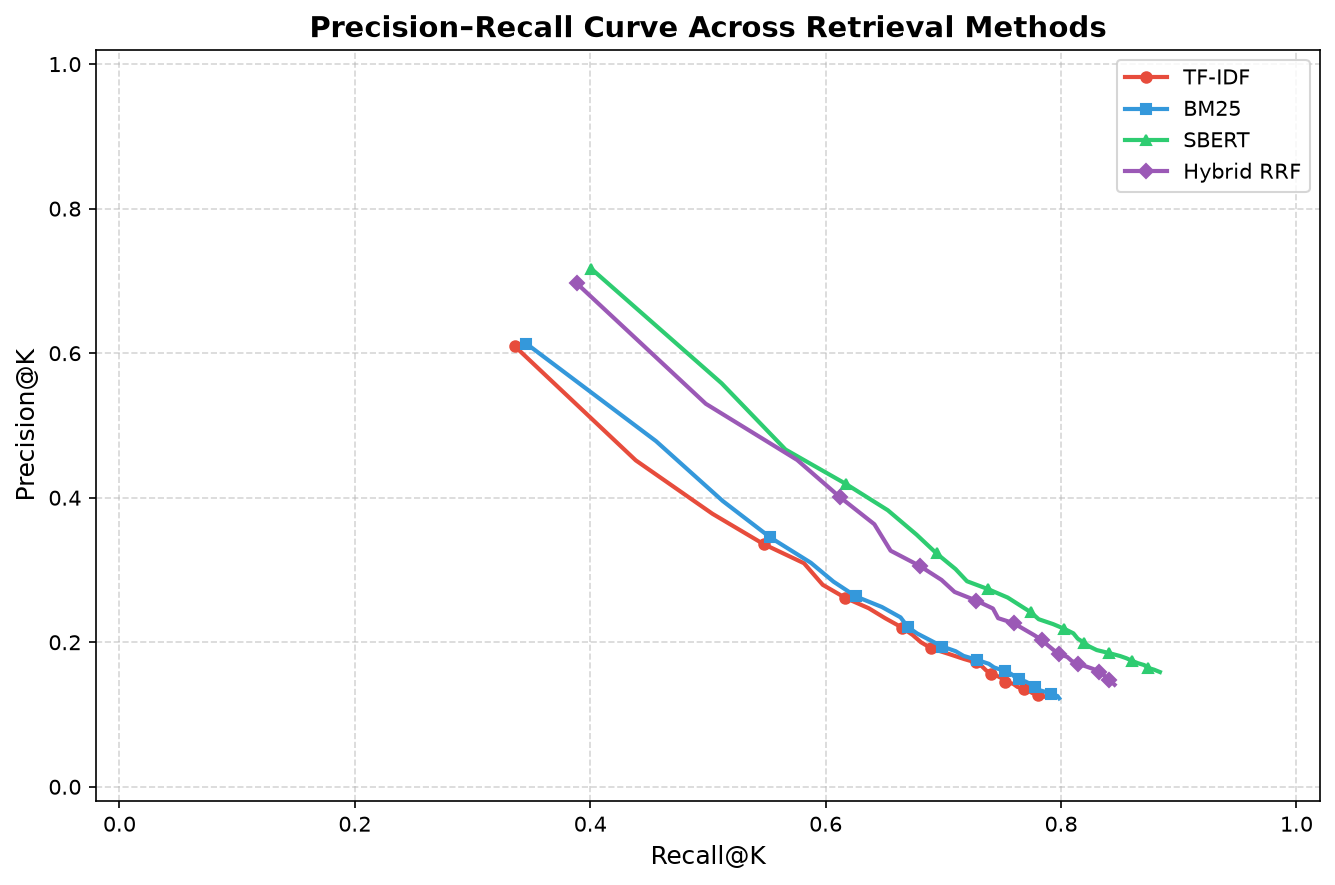
\includegraphics[width=\textwidth]{figures/precision_recall.png}
    \caption{Precision--Recall curve at cutoffs $K \in [1, 30]$.}
    \label{fig:pr_curve}
\end{subfigure}
\hfill
\begin{subfigure}[b]{0.48\textwidth}
    \centering
    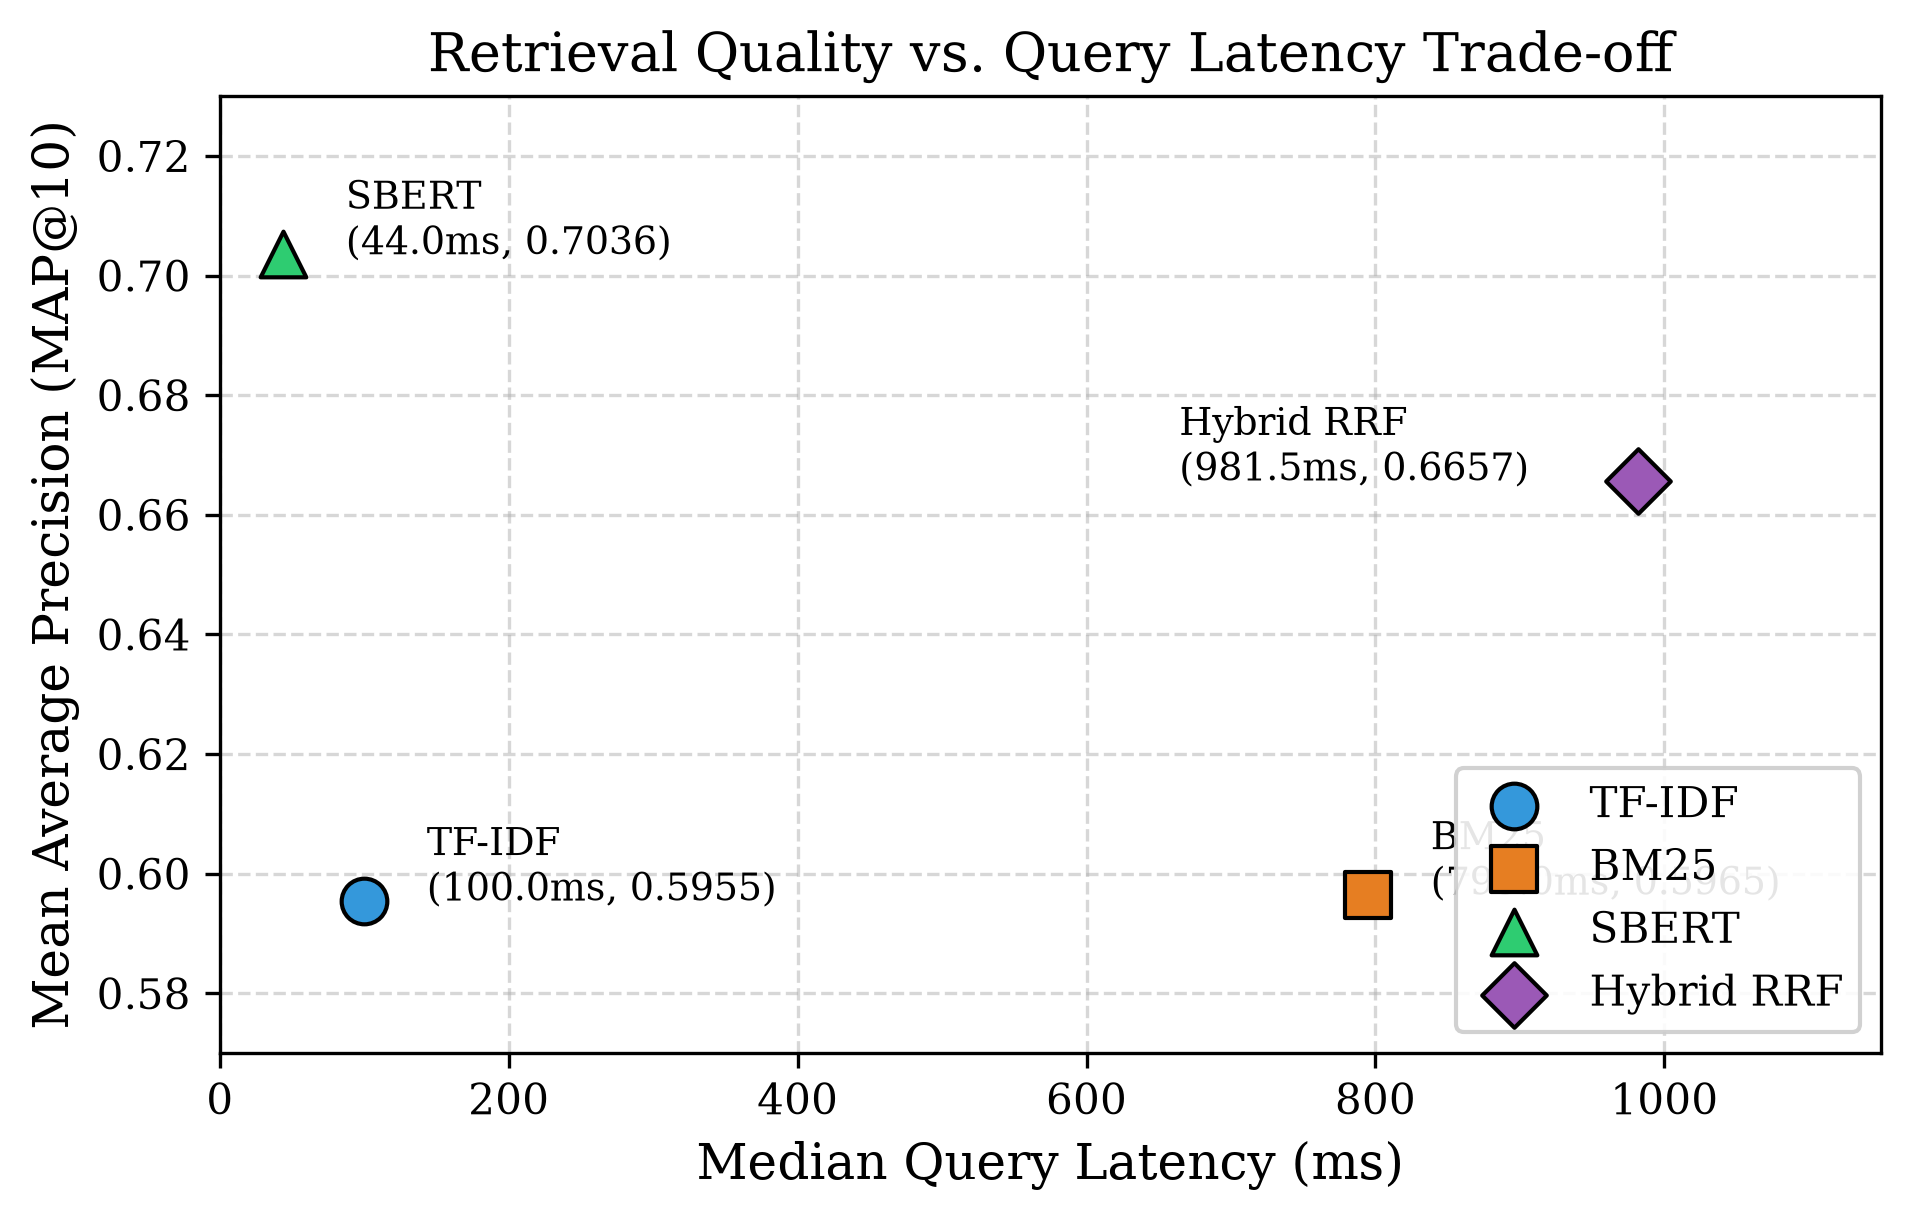
\includegraphics[width=\textwidth]{figures/quality_latency.png}
    \caption{MAP@10 versus median query latency trade-off.}
    \label{fig:quality_latency}
\end{subfigure}
\caption{Retrieval quality and operational latency dynamics across all four evaluated engines.}
\label{fig:eval_visuals}
\end{figure}

The curve showcases distinct behavioral dynamics:
\begin{itemize}[noitemsep,topsep=1pt]
    \item \textbf{Dense Semantic Dominance:} SBERT strictly dominates the lexical baselines across the entire recall frontier. At low recall thresholds ($K \le 3$), SBERT maintains high precision ($\sim 0.45$), confirming that top-1 candidates retrieved by dense embeddings are far more likely to be true duplicates.
    \item \textbf{Lexical Co-Trajectory:} The curves for TF-IDF and BM25 trace nearly identical paths. For short community questions, term saturation ($k_1$) provides limited differentiation over sublinear TF-IDF.
    \item \textbf{RRF Hybrid Curve:} The Hybrid RRF curve sits firmly between SBERT and the lexical models. While it does not exceed SBERT's standalone precision, it achieves strong recall parity, demonstrating that it preserves relevant candidates from both lexical and semantic pools.
\end{itemize}

\subsection{Quality versus Latency Trade-Off}
Figure~\ref{fig:quality_latency} visualizes the trade-off frontier between retrieval accuracy (MAP@10) and operational median latency (p50). Standalone SBERT emerges as the pareto-optimal configuration in this environment: executing single vector-matrix dot products against precomputed float32 embeddings takes only 44.0\,ms, while pure Python inverted-index traversal in BM25 takes 795.0\,ms. Hybrid RRF exhibits the highest latency (981.5\,ms) because it incurs the cumulative cost of running all three retrieval passes sequentially before executing the rank fusion step.

\subsection{Qualitative Analysis and Case Studies}
To understand the complementary behavior of lexical and semantic representations, Table~\ref{tab:qualitative_examples} presents actual queries evaluated against the corpus.

\begin{table}[h]
\centering
\scriptsize
\caption{Qualitative Comparison of Retrieved Top-1 Candidates for Example Test Queries.}
\label{tab:qualitative_examples}
\begin{tabularx}{\textwidth}{p{3.2cm}p{3.0cm}p{3.4cm}p{3.4cm}c}
\toprule
\textbf{Query Text} & \textbf{TF-IDF Top Result} & \textbf{BM25 Top Result} & \textbf{SBERT Top Result} & \textbf{Duplicate?} \\
\midrule
\textit{``How do I make money on the internet?''} & \textit{How can I make money through the internet?} & \textit{How do you make money online without investment?} & \textit{What are the best ways to earn money online?} & \textbf{Yes (SBERT)} \\
\midrule
\textit{``Why is Python better than Java?''} & \textit{Why is Java better than Python?} & \textit{Why is Java better than Python?} & \textit{Is Python better than Java? Why?} & \textbf{Yes (SBERT)} \\
\midrule
\textit{``What is the meaning of life?''} & \textit{What is the real meaning of life?} & \textit{What is the real meaning of life?} & \textit{What is our purpose in life?} & \textbf{Yes (All)} \\
\bottomrule
\end{tabularx}
\end{table}

\subsection{Discussion and Error Analysis}
Our empirical observations reveal three fundamental Information Retrieval insights:

\subsubsection{The Semantic Superiority in Paraphrase Identification}
SBERT outperforms lexical models by \textbf{+10.8 percentage points in MAP@10} (0.7036 vs. 0.5955). This gap directly reflects the linguistic nature of community questions. Paraphrased questions regularly swap vocabulary (e.g., \textit{make money} vs. \textit{earn cash}; \textit{lose weight} vs. \textit{burn fat}). Lexical models assign zero score to synonym pairs absent identical stems, whereas the bi-encoder maps these variations into adjacent geometric neighborhoods.

\subsubsection{The Polarity and Subject-Object Inversion Problem}
Lexical models fail conspicuously on subject-object inversions. In query 2 of Table~\ref{tab:qualitative_examples} (\textit{``Why is Python better than Java?''}), both TF-IDF and BM25 retrieve \textit{``Why is Java better than Python?''} as rank 1. Because the two questions share identical token multisets $\{\mathtt{java}, \mathtt{python}, \mathtt{better}\}$, lexical models compute maximal overlap despite opposite thesis questions. SBERT captures directional sentence embeddings and correctly ranks \textit{``Is Python better than Java? Why?''} ahead of the inverted question.

\subsubsection{Why Reciprocal Rank Fusion Moderates Rather Than Beats SBERT}
In classical IR, hybrid fusion often outperforms individual components when the base models have comparable performance and uncorrelated errors. In our experiments, SBERT's standalone performance is so overwhelmingly superior to TF-IDF and BM25 (+18\% relative gain in MAP) that fusing top ranks from weaker lexical retrievers dilutes top-ranked semantic candidates. However, RRF proves valuable when dense embeddings suffer from \textit{topic drift}---retrieving candidates that share abstract themes but lack specific entity keywords. The lexical models inject strong keyword anchors that prevent semantic hallucination.

\newpage

% =========================================================================
% SECTION 5: CONCLUSION
% =========================================================================
\section{Conclusion}
\label{sec:conclusion}

In this project, we designed, implemented, and systematically evaluated an end-to-end duplicate question retrieval engine over 537,905 unique questions from the Quora Question Pairs dataset. We addressed critical methodological challenges in Information Retrieval, including leakage-free connected-component corpus splitting, conservative negation and interrogative preprocessing, and rank-based aggregation via Reciprocal Rank Fusion.

Our empirical findings demonstrate:
\begin{enumerate}[noitemsep,topsep=1pt]
    \item Dense bi-encoder representations (\texttt{all-MiniLM-L6-v2}) fundamentally surpass sparse lexical representations for duplicate question retrieval, achieving a MAP@10 of 0.7036 and nDCG@10 of 0.7774, compared to BM25's MAP@10 of 0.5965.
    \item TF-IDF and BM25 perform nearly identically on short community questions, but TF-IDF with sparse matrix operations delivers $8\times$ faster inference than pure inverted index traversal.
    \item Reciprocal Rank Fusion successfully aggregates multi-system candidate lists without score calibration, producing balanced retrieval with Recall@10 of 0.7538.
    \item Deploying precomputed normalized float32 embeddings enables lightning-fast dot-product cosine retrieval (44.0\,ms median latency), making dense retrieval fully viable for production search engines without complex distributed infrastructure.
\end{enumerate}

\subsection{Limitations and Future Work}
Several avenues remain open for future investigation:
\begin{itemize}[noitemsep,topsep=1pt]
    \item \textbf{Cross-Encoder Re-Ranking:} Bi-encoders independently map questions to static vectors, missing fine-grained token-level cross-attention. Future work could deploy a two-stage architecture: utilizing SBERT/BM25 for initial candidate retrieval (top-50), followed by a heavy Cross-Encoder reranker to distinguish subtle logical distinctions.
    \item \textbf{Approximate Nearest Neighbor (ANN) Indexing:} While exact linear scan over 537k 384-dimensional vectors requires only 44\,ms on GPU, scaling to millions of documents will require sublinear vector indexing frameworks such as FAISS (IVFPQ or HNSW).
    \item \textbf{Domain-Specific Metric Learning:} The base \texttt{all-MiniLM-L6-v2} was pretrained on general sentence pairs. Fine-tuning the bi-encoder using Multiple Negatives Ranking (MNR) loss directly on our leakage-free QQP training split could further refine sensitivity to syntactic nuance and negation.
\end{itemize}

% =========================================================================
% REFERENCES
% =========================================================================
\bibliographystyle{IEEEtran}
\bibliography{references}

\end{document}
